 \documentclass[12pt]{article}
\usepackage[spanish, mexico]{babel} % espanol
\usepackage[utf8]{inputenc} % acentos sin codigo
\usepackage{enumerate} % enumerados
\usepackage{amsmath}
\usepackage{amsfonts}
\usepackage{amssymb}
\usepackage{graphicx}
\usepackage{float}

\title{Actividad 1}
\author{Paulina Valenzuela Coronado}
\date{Enero 2016}
\begin{document}
\maketitle

\section{El Péndulo}
\subsection{Péndulo Simple}
está constituido por un hilo inextensible de masa despreciable, sostenido por su extremo superior de un punto fijo, con una masa puntual sujeta en su extremo inferior que oscila libremente en un plano vertical fijo.
El movimiento solo ocurre en dos dimensiones y este no pierde energía por la fricción o la resistencia del aire.\cite{Wiki} \\

La ecuación del movimiento de un péndulo simple es 

\begin{equation}
\frac{
d^2\theta}{dt^2}+\frac{g}{l}\sin\theta=0
\end{equation}

donde
\begin{itemize}
\item $g$ es la aceleración debida a la gravedad
\item $l$ es el lago del péndulo
\item $\theta$ es el desplazamiento angular 
\end{itemize}

\begin{figure}[H]
	\centering
\includegraphics[width=5cm]{12.png}
 \caption{Péndulo simple}
\end{figure} 

\subsection{Método 1 "Fuerza"}		
La figura 2 muestra las fuerzas actuando en un péndulo simple. Observe que la trayectoria del péndulo es un arco de un círculo, el angulo $\theta$ está medido en radianes.	

\begin{figure}[H]
   \centering
	\includegraphics[width=5cm]{5.png}
	\caption{Diagrama de fuerzas en un péndulo simple}
\end{figure}
        
Considere la segunda ley de Newton
$$F=ma$$
donde 
\begin{itemize}
	\item $F$ es la suma de las fuerzas en el objeto
	\item $m$ es la masa
	\item $a$ es la aceleración
\end{itemize}

Ya que solo consideramos los cambios en la velocidad, ya que la masa esta forzada a una trayectoria circular, aplicamos la ecuación de Newton para un eje tangencial.

Entonces
\begin{eqnarray}
\nonumber F & = & -mg\sin\theta =ma \\
\nonumber a & = & -g\sin\theta
\end{eqnarray}

donde $g$ es la aceleración por la gravedad cerca de la superficie de la tierra.
El signo negativo implica que $\theta$ y $a$ siempre van en direcciones opuestas.

La aceleración lineal $a$ a lo largo del eje rojo puede ser relacionada con el cambio en el angulo $\theta$ por las fórmulas de la longitud de arco, $s$ es la longitud de arco:

\begin{eqnarray}
\nonumber s &  = & l\theta \\
\nonumber v & = & \frac{ds}{dt}  =  l\frac{d\theta}{dt} \\
\nonumber a  & = &  \frac{d^2s}{dt^2}  =  l\frac{d^2\theta}{dt^2}
\end{eqnarray}

Asi 
 \begin{eqnarray}
 \nonumber l \frac{d^2s}{dt^2} = -g \sin\theta \\
 \nonumber  \frac{d^2s}{dt^2} + \frac{g}{l} \sin \theta =  0
 \end{eqnarray}

 \subsection{Método 2 "Torca"}
 La ecuación (1) puede ser obtenida usando dos definiciones de torca.
 $$ \tau = r xF = \frac{dL}{dt}$$ 
 Primero define la torca de un péndulo usando la fuerza debida a la gravedad
 
\begin{eqnarray}
\nonumber \tau & = & l x F_g \\
\nonumber |\tau| & = & -mgl\sin\theta
\end{eqnarray}

donde 
\begin{itemize}
\item $l$ es el vector longitud de el péndulo
\item $F_g$ es la fuerza debida a la gravedad
\item $m$ es la masa del péndulo
\item $g$ es la aceleración de la gravedad
\item $\theta$ es el angulo entre el vector longitud  y la fuerza debida a la gravedad
\end{itemize}

Rescribiendo el momento angular

\begin{eqnarray}
\nonumber L & = & r x p = mr x (\omega x r) \\
\nonumber |L| & = & mr^2 \omega = ml^2 \frac{d\theta}{dt} \\
\nonumber \frac{d}{dt} |L|&  = & ml^2\frac{d^2\theta}{dt^2} 
\end{eqnarray}

Como $\tau = \frac{dL}{dt}$ podemos comparar magnitudes


$$ -mgl\sin\theta =  ml^2\frac{d^2\theta}{dt^2} $$

Entonces 

\begin{equation}
\nonumber \frac{d^2\theta}{dt^2}+\frac{g}{l}\sin\theta=0
\end{equation}

\subsection{Método 3 "Energía"}
Esta ecuación también se puede obtener a partir del principio de  la conservación de la energía mécanica: cualquier objeto cayendo en una distancia vertical $h$ adquiriría energía cinética igual a la que se perdió con la caída. En otras palabras, la energía potencial gravitatoria se convierte en energía cinética. El cambio en la energía potencial está dado por 
$$\Delta U = mgh$$ 
Y el cambio en la energía cinética se define como:
$$\Delta K = \frac{1}{2}mv^2$$
Dado que no se pierde energía, la ganancia en un solo debe ser igual a la pérdida en el otro

$$\frac{1}{2}mv^2=mgh$$

El cambio de velocidad para un cambio dado en la altura se puede expresar
$$v=\sqrt{2gh}$$

Utilizando la fórmula de la longitud del arco anterior, esta ecuación puede reescribirse en términos de $\frac{d\theta}{dt}$
$$v=l\frac{d\theta}{dt}=\sqrt{2gh}$$
$$\frac{d\theta}{dt}= \frac{1}{l}\sqrt{2gh}$$

donde $h$ es la distancia vertical donde el péndulo cae.

\begin{figure}[H]
	\centering
	\includegraphics[width=6cm]{11.png}
	\caption{Trigonometría de un péndulo simple}
\end{figure}

Observe la figura 2, que presenta la trigonometría de un péndulo simple. Si el péndulo comienza su oscilación de algun $\theta_0$ de ángulo inicial, entonces $y_0$, la distancia vertical desde el tornillo, está dada por
$Y_0=l\cos\theta_0$
Para $y_1$ tenemos
$Y_1=l\cos\theta$
Entonces $h$ es la diferencia de los dos
$h=l(\cos\theta-\cos\theta_0)$
en términos de $\frac{d\theta}{dt}$

\begin{equation}
\nonumber \frac{d\theta}{dt}=\sqrt{\frac{2g}{l}(\cos\theta-\cos\theta_0)}
\end{equation}

Esta ecuación es conocida como la primera integral de movimiento, está ecuación nos da la velocidad en términos de la posición e incluye una integración constante relacionada con el desplazamiento incial $(\theta_0)$. podemos aplicar la regla de la cadena, con respecto al tiempo para obtener la aceleración:

$\frac{d}{dt}\frac{d\theta}{dt}=\frac{d}{dt}\sqrt{\frac{2g}{l}(\cos\theta-\cos\theta_0)}$\\
	
$\frac{d^2\theta}{dt^2}=\frac{1}{2} \frac{-(\frac{2g}{l}\sin\theta)}{\sqrt{\frac{2g}{l}(\cos\theta-\cos\theta_0)}}\frac{d\theta}{dt}$	\\	
	
$=\frac{1}{2}\frac{-(\frac{2g}{l}\sin\theta)}{\sqrt{\frac{2g}{l}(\cos\theta-\cos\theta_0)}}\sqrt{\frac{2g}{l}(\cos\theta-\cos\theta_0)}=\frac{-g}{l}\sin\theta$ \\
			
$\frac{d^2\theta}{dt^2}+\frac{g}{l}\sin\theta = 0$ \\

que es el mismo resultado que obtiene a través de análisis de fuerzas.

	
\section{Aproximación con angulos pequeños}
No hay solución de la ecuación anterior que pueda ser escrita por funciones elementales, pero dandole una restricción al tamaño de la amplitud de la oscilación entonces da una forma cuya solución se puede obtener fácilmente. Si supone que el ángulo es mucho menor que 1 radián, o $$\theta  \ll 1$$ entonces sustituyendo por $\sin \theta$ en la ecuación 1, usando esta aproximación $$\sin \theta \equiv\theta$$ se obtiene la ecuación para un oscilador armónico.
 \begin{equation}
 \nonumber \frac{d^2\theta}{dt^2}+\frac{g}{l}\theta=0
 \end{equation}

El error debido a la aproximación es del orden de $\theta^3$.
Dadas las condiciones iniciales $\theta(0)=\theta_0$ y $\frac{d\theta}{dt}(0)=0$, la solución se convierte

\begin{equation}
\nonumber \theta(t)= \theta_0 (\sqrt{\frac{g}{l}t})  \qquad \theta_0 \ll 1
\end{equation}

El período del movimiento, el tiempo en completar una oscilación es

\begin{equation}
\nonumber T(0)= 2\pi \sqrt{\frac{l}{g}} \qquad \theta_0 \ll 1
\end{equation}

Esta ecuacción es conocida como la ley de Christiaan Huygens para el período. Observe que bajo la aproximación para angulos pequeños, el período es independiente de la amplitud $\theta_0$, esto es una propiedad del isocronismo que Galileo descubrió.

\subsection{Regla del oro para la longitud de un péndulo}
$T(0)= 2\pi \sqrt{\frac{l}{g}}$ puede ser expresado como $l= \frac{g}{\pi^2} x \frac{T_0^2}{4}$
	
Considerando que las medidas son tomadas en la superficie de la tierra, entonces $g \approx 9.81 \frac{m}{s^2}$ y $\frac{g}{\pi^2} \approx 1$ 

Por lo tanto, una aproximación razonable para el largo y el período son:

\begin{eqnarray}
\nonumber l & \approx & \frac{T_0^2}{4} \\
\nonumber T_0 & \approx & 2 \sqrt{l}
\end{eqnarray} 

Donde $T_0$ es el número de segundos entre dos pulsos y $l$ es una medida en metros.

\section{Período con Amplitud Arbitraria}
Para amplitudes fuera de la aproximación de angulos pequeños se puede computarizar el período exacto, invirtiendo la ecuación para la velocidad angular obtenida del método de la energía.


\begin{figure}[H]
	\centering
	\includegraphics[width=6cm]{8.png}
	\caption{Desviación del verdadero período}
\end{figure}

\begin{figure}[H]
	\centering
	\includegraphics[width=6cm]{2.png}
	\caption{Diagrama de fuerzas en un péndulo simple}
\end{figure}



$$\frac{dt}{d\theta} = \frac{l}{2g} \frac{1}{\cos \theta - \cos \theta_0} $$
Integrando sobre un ciclo completo
$$T=t(\theta_0 \rightarrow 0 \rightarrow -\theta_0 \rightarrow 0 \rightarrow \theta_0)$$,

o dos veces para medio ciclo
$$T=2t(\theta_0 \rightarrow 0 \rightarrow -\theta_0)$$,

o cuatro veces para un cuarto de ciclo

$$T=4t(\theta_0 \rightarrow 0)$$,

Lo que lleva a 

$$T= 4\sqrt{\frac{l}{2g}} \int_{0}^{\theta_0}\frac{1}{\cos \theta - \cos \theta_0}d\theta$$.

Observe que esta integral diverge a $\theta_0$ aproximandose a la vertical

$$\lim\limits_{\theta_0\to\pi} T = \infty$$.

Esta integral puede ser reescrita en términos de integrales elipticas como

$$T= 4 \sqrt{\frac{l}{g}} F(\frac{\theta_0}{2}, \csc\frac{\theta}{2})\csc\frac{\theta}{2}$$

Donde $F$ es la integral elíptica incompleta de la primera clase definida por

$$F(\varphi, k) = \int_{0}^{\varphi} \frac{1}{\sqrt{1-k^2\sin^2u}} du$$.

O más concisamente por la sustitución $\sin u = \frac{\sin \frac{\theta}{2}}{\sin \frac{\theta_0}{2}}$ expresando $\theta$ en términos de $u$,
\begin{equation}
\nonumber T= 4 \sqrt{\frac{l}{g}}K(\sin^2 (\frac{\theta_0}{2})
\end{equation}
donde $K$ es una integral elíptica completa de la primera clase definida por

$$K(k)0 F (\frac{\pi}{2},k)=\int_{0}^{\frac{\pi}{2}}\frac{1}{\sqrt{1-k^2\sin^2u}} du$$.

Desde aquí hay muchas formas de resolver la integral elíptica:

\subsection{Solución de un polinomio de Legendre para la integral elíptica}
Dada la ecuación (3) y la solución Legendre polinomial para la integral elíptica:

$K(k)=\frac{\pi}{2}\{1+(\frac{1}{2})^2 k^2 + (\frac{1 \cdot 3 }{2 \cdot 4})^2k^4 + ...+ [\frac{(2n-1)!!}{(2n)!!}]^2k^{2n}+...\}$

Donde $n!!$ denota doble factorial, una solución exacta del período de un péndulo es:
\begin{eqnarray}
\nonumber T & = & 2\pi\sqrt{\frac{l}{g}} (1+(\frac{1}{2})^2\sin^2 (\frac{\theta_0}{2})+(\frac{1 \cdot 3 }{2 \cdot 4})^2\sin^4(\frac{\theta}{2})+(\frac{1 \cdot 3 \cdot 5}{2 \cdot 4 \cdot 6})^2\sin^6(\theta_0)+...) \\
\nonumber & = & 2\pi \sqrt{\frac{l}{g}} \sum_{n=0}^{\infty}[(\frac{(2n)!}{(2^n \cdot n!)^2})^2 \cdot \sin^2n(\frac{\theta_0}{2})]
\end{eqnarray}

La figura 4 muestra los errores relativos usando series de potencia. $T_0$ es una aproximación lineal, y $T_2$ a $T_10$ incluyendo respectivamente los términos hasta el 2do y 10mo.

\begin{figure}[H]
	\centering
	\includegraphics[width=6cm]{2.png}
	\caption{Errores relativos usando series de potencia}
\end{figure}

\subsection{Solución en serie de potencias de la integral elíptica}
Otra formulación de la solución anterior se puede encontrar con la siguiente serie de Maclaurin:

$$\sin\frac{\theta_0}{2}=\frac{1}{2}\theta_0 - \frac{1}{48}\theta_0^3+\frac{1}{3840}\theta_0^5-\frac{1}{345120}\theta_0^7+...$$
se ultiliza en la solución polinomial de Legendre. La serie de potencia que resulta es:

$T=2\pi\sqrt{\frac{l}{g}}(1+\frac{1}{16}\theta_0^2+\frac{11}{3072}\theta_0^4+\frac{173}{737280}\theta_0^6+\frac{22931}{1321205760}\theta_0^8+\frac{1319183}{951268147200}\theta_0^{10}+\frac{233526463}{2009078326886400}\theta_0^{12}+...)$

\begin{figure}[H]
	\centering
	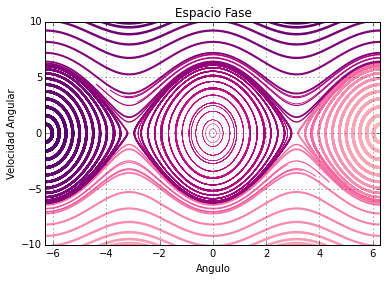
\includegraphics[width=6cm]{3.png}
	\caption{Energía Potencial y retrato fase de un péndulo simple.}
\end{figure}

\subsection{Solución media aritmética-geométrica para la integral elíptica}

Dada la ecuación (3) y la solución media aritmética-geométrica de la integral elíptica:

$$K(k)=\frac{\frac{\pi}{2}}{M(1-k,1+k)}$$

donde $M(x,y)$ es la  media aritmética-geométrica de $x$ y $y$.
Esto produce una fórmula alternativa y que converge más rápido para el período:

$$T=\frac{2\pi}{M(1,cos(\frac{\theta_0}{2}))}\sqrt{\frac{l}{g}}$$

\begin{thebibliography}{9}
	
	\bibitem{Wiki}
Wikipedia en Español, https://es.wikipedia.org/wiki/P%C3%A9ndulo
	\emph{Péndulo}
	
	\bibitem{Wikipedia}
	https://en.wikipedia.org/wiki/Pendulum_%28mathematics%29

   \bibitem{}	
\end{thebibliography}



\end{document}